\chapter{TRABALHOS RELACIONADOS} 
\label{chap:trab_relacionados}

% Neste capítulo serão apresentados trabalhos correlatos a este em ordem cronológica de
% publicação. Cada seção é referente a um tópico desta pesquisa, sendo as duas primeiras (Seções
% 3.1 e 3.2), segmentação e classificação, relacionadas a tarefas de visão computacional e divididas entre trabalhos envolvendo a criação de bases de dados (Seções 3.1.1 e 3.2.1) e de modelos
% (Seções 3.1.2 e 3.2.2) para cada um dos tópicos em questão. A Seção 3.3, reconhecimento automático de dor em recém-nascidos, traz algumas das abordagens criadas em função dos anos,
% para contextualização sobre as técnica disponíveis no meio.

Aplicar a unificação de técnicas radiômicas e aprendizado profundo na pesquisa de cardiomiopatia tem recebido cada vez mais atenção da comunidade científica.
Neste capítulo serão apresentados trabalhos e metodologias correlatos ao esforço de outros autores a cerca deste tema. Será descrito como foi a metodologia utilizada na revisão sistemática da literatura \cite{petersenGuidelinesConductingSystematic2015a}, assim como trabalhos que trazem ideias próximas ao proposto neste trabalho.

%---------------------------------------------------------
\section{Revisão Sistemática da Literatura} 
\label{sec:rev_sistematica}

Para a fase exploratória dos trabalhos relacionados, foi utilizada a ferramenta \textit{Parsifal} \footnote{https://parsif.al} com o objetivo de identificar estudos que aplicam a análise radiômica no contexto de cardiomiopatia. O objetivo inicialmente definido foi o seguinte: ``Identificar estudos onde se aplica análise radiômica a cardiopatia. Em segunda opção, alguma outra doença de natureza cardíaca''. A pesquisa teve como objetivo responder as seguintes perguntas: quais desafios descritos nos estudos prévios e se há replicabilidade da proposta. As palavras chaves selecionadas foram: \textit{cardiac}, \textit{cardiomyopathy} e \textit{radiomics}. A palavra de busca selecionada foi: ``\textit{radiomics} AND (\textit{cardiac} OR \textit{cardiomyopathy})''. Os resultado do filtro de busca são apresentados na Tabela \ref{tab:resultado_busca}. 
\newline

\begin{table}[hbtp]
    \caption{Resultados dos Artigos}
    \centering
    \renewcommand{\arraystretch}{1.4} % default é 1 
    \begin{tabular}{|c|c|}
    \hline 
          \textbf{Origem} & \textbf{Artigos}  \\ 
    \hline 
        IEEE & 6 \\ 
        PUBMED & 19 \\ 
        Science@Direct & 24 \\ 
    \hline 
    \end{tabular} 
    \caption*{Fonte: Autor}
    \label{tab:resultado_busca}
\end{table}

A partir dos resultados foram aplicados os critérios de inclusão e exclusão conforme descritos na Tabela \ref{tab:criterios}.

\begin{table}[hbtp]
    \centering
    \caption{Critérios de Inclusão e Exclusão}
    \renewcommand{\arraystretch}{1.4} % default é 1 
    \begin{tabular}{|l|l|}
    \hline 
          \multicolumn{1}{|c|}{\textbf{Critério de Inclusão}} & \multicolumn{1}{c|}{\textbf{Critério de Exclusão}}  \\ 
    \hline 
        \quad Contém ressonância magnética? & \quad Estudos Duplicados   \\ 
        \quad O objeto de estudo é o coração? & \quad Estudos Secundários ou Terciários \\
        \quad Usa análise de textura? & \quad Estudos que não estão em PT ou EN\\
        \quad Utiliza análise radiômica? & \quad Leitura cinza  \\
        \quad É cardiomiopatia? & \quad Não aplica técnicas computacionais\\
        & \quad Não trata do coração \\
        & \quad Não usa RM \\
        & \quad Trabalho que atua somente com dados genômicos \\ 
    \hline 
    \end{tabular} 
    \caption*{Fonte: Autor}
    \label{tab:criterios}
\end{table}

Critérios de inclusão também foram aplicados e são apresentados na Tabela \ref{tab:questoes}. Dentre estes critérios, cada artigo é representado pela soma das pontuações obtidas pelos critérios e os artigos que obtiveram uma nota menor que 3 foram excluídos da revisão. Para as notas, ficou definido como pontuação: $1$ para critério aceito, $0,5$ para critério parcialmente aceito e $0$ para critério não atingido. Uma vez aplicado os critérios e filtrado mediante pontuação, restaram $18$ dos $49$ artigos iniciais.


\begin{table}[hbtp]
    \centering
    \caption{Questões de Aceitação}
    \renewcommand{\arraystretch}{1.4} % default é 1 
    \begin{tabular}{|l|}
    \hline 
          \multicolumn{1}{|c|}{\textbf{Questões}} \\ 
    \hline 
        \quad É descrita as limitações do estudo? \\
        \quad Há um experimento bem descrito para avaliar a proposta? \\
        \quad Há mais de 2 autores? \\
        \quad O trabalho apresenta resultados? \\
        \quad A introdução apresenta o problema de forma clara \\
        \quad É análise sistemática da literatura? \\
    \hline 
    \end{tabular} 
    \caption*{Fonte: Autor}
    \label{tab:questoes}
\end{table}

O diagrama com o funil de seleção aplicado é apresentado na Figura \ref{fig:fig021}. É possível verificar na imagem, por exemplo, que foram removidos $28$ artigos dos $49$ artigos selecionados inicialmente, restando $21$. Aplicando os critérios de qualidade, foram selecionados $18$ artigos. Dentre os artigos selecionados, $3$ foram excluídos por não agregarem o suficiente ou por serem redundantes.

\textcolor{red}{
< < ----- MENCIONO QUE ADICIONEI 2 LITERATURAS POSTERIORES ??? -----
}

Por fim, duas novas literaturas foram adicionadas as já elencadas pela revisão sistemática. Isto ocorre na fase em que são feitos diversos testes e coletados os resultados, mediante diversas interações, abordagens como o \gls{SE}-Net foram identificadas e, dada sua revisão, incorporadas ao modelo base utilizado obtendo resultados significativamente superiores se comparados ao do modelo base.


\textcolor{red}{
-------------------------------------------------------------------------------------------- > >
}

\begin{figure}[h!]
    \centering
    \caption{Funil da Seleção da Literatura}
    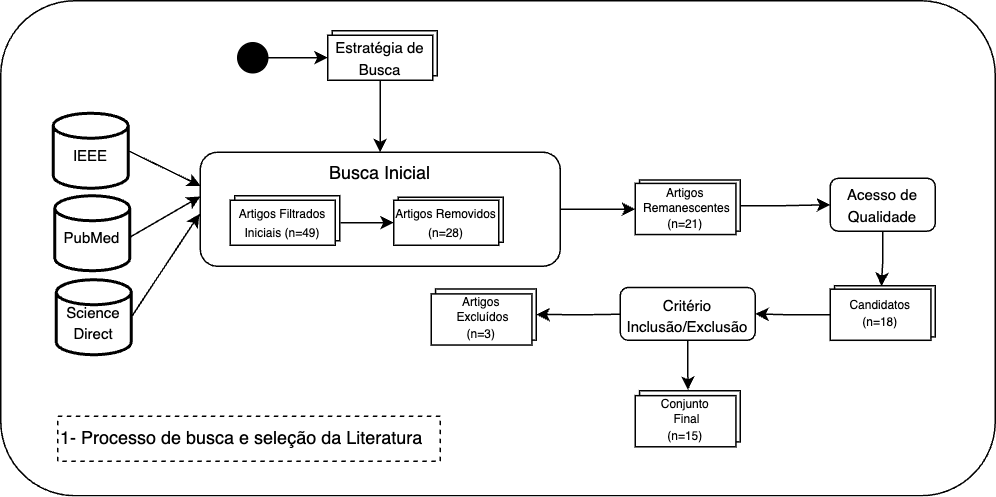
\includegraphics[scale=0.47]{figures/fig021.png}
    \caption*{Fonte: Autor}
    \label{fig:fig021}
\end{figure}

%---------------------------------------------------------
\section{Análise Radiômica com Atenção}
\label{sec:analise_radiomica}

\citeonline{jiangMRIBasedRadiomics2021} conduziram um estudo abrangente que aproveita as capacidades do aprendizado de máquina para melhorar os processos diagnósticos em oncologia, especificamente focando no câncer de colo de útero em estágio inicial. Sua pesquisa, intitulada ``Abordagem Radiômica Baseada em Ressonância Magnética com Aprendizado Profundo para Predição de Invasão Vascular em Câncer de Colo de Útero em Estágio Inicial'', foca na aplicação de técnicas de aprendizado profundo em dados de \gls{RMC} multiparamétrica para prever a invasão vascular, um fator crítico para determinar a agressividade do câncer de colo de útero e informar estratégias de tratamento.

O estudo utilizou um conjunto substancial de dados compreendendo $1.070$ imagens de ressonância magnética com contraste dinâmico T1 (DCE-T1) e $986$ imagens de ressonância magnética ponderadas em T2 (T2WI) e coletadas de $167$ pacientes diagnosticadas com câncer do colo do útero em estágio inicial entre janeiro de $2014$ e agosto de $2018$. Os pesquisadores empregaram uma nova estrutura de aprendizado profundo que integrou esses dois tipos distintos de varreduras em imagens de \gls{RMC} para criar um modelo preditivo robusto. Implementando uma estratégia de aprendizado em conjunto com atenção, o modelo efetivamente distinguiu entre casos com invasão vascular e aqueles sem. Quatro modelos de CNN foram utilizados: VGGNet, GoogLeNet (Inception-v3), Residual Network (ResNet) e \textit{DenseNet}. Um módulo padrão de \gls{SE}  e o módulo de atenção de bloco convolucional, do termo inglês \gls{CBAM},  foram introduzidos após cada bloco de convolução da rede \textit{AdaptedVGG19} para fornecer um \textit{AdaptedVGG19-SE} e um \textit{AdaptedVGG19-CBAM}, respectivamente. A arquitetura proposta é vista na Figura \ref{fig:fig007}.

O desempenho preditivo dos modelos foi rigorosamente avaliado, com os modelos finais alcançando uma \gls{AUC} de 0,911. Essa alta \gls{AUC} indica uma forte capacidade do modelo para classificar corretamente a presença ou ausência de invasão vascular, com métricas de sensibilidade e especificidade também demonstrando precisão diagnóstica substancial.

Esta pesquisa demonstra o potencial de integrar algoritmos de aprendizado profundo com dados de imagem complexos para melhorar as avaliações diagnósticas pré-operatórias. Os achados de \citeonline{jiangMRIBasedRadiomics2021} sugerem que tais abordagens analíticas avançadas podem fornecer suporte substancial na tomada de decisões clínicas, potencialmente levando a planos de tratamento mais personalizados e melhores resultados para os pacientes.

No contexto da pesquisa contínua em imagens médicas e diagnóstico de câncer, a metodologia e os resultados fornecem um exemplo convincente do potencial da inteligência artificial para revolucionar os processos diagnósticos em oncologia. O uso de \gls{RMC} multiparamétrica e modelos sofisticados de aprendizado de máquina exemplifica as abordagens inovadoras que estão sendo desenvolvidas para enfrentar os desafios da detecção precoce e precisa de câncer.

\begin{figure}[htbp]
    \centering
    \caption{Arquitetura Proposta}
    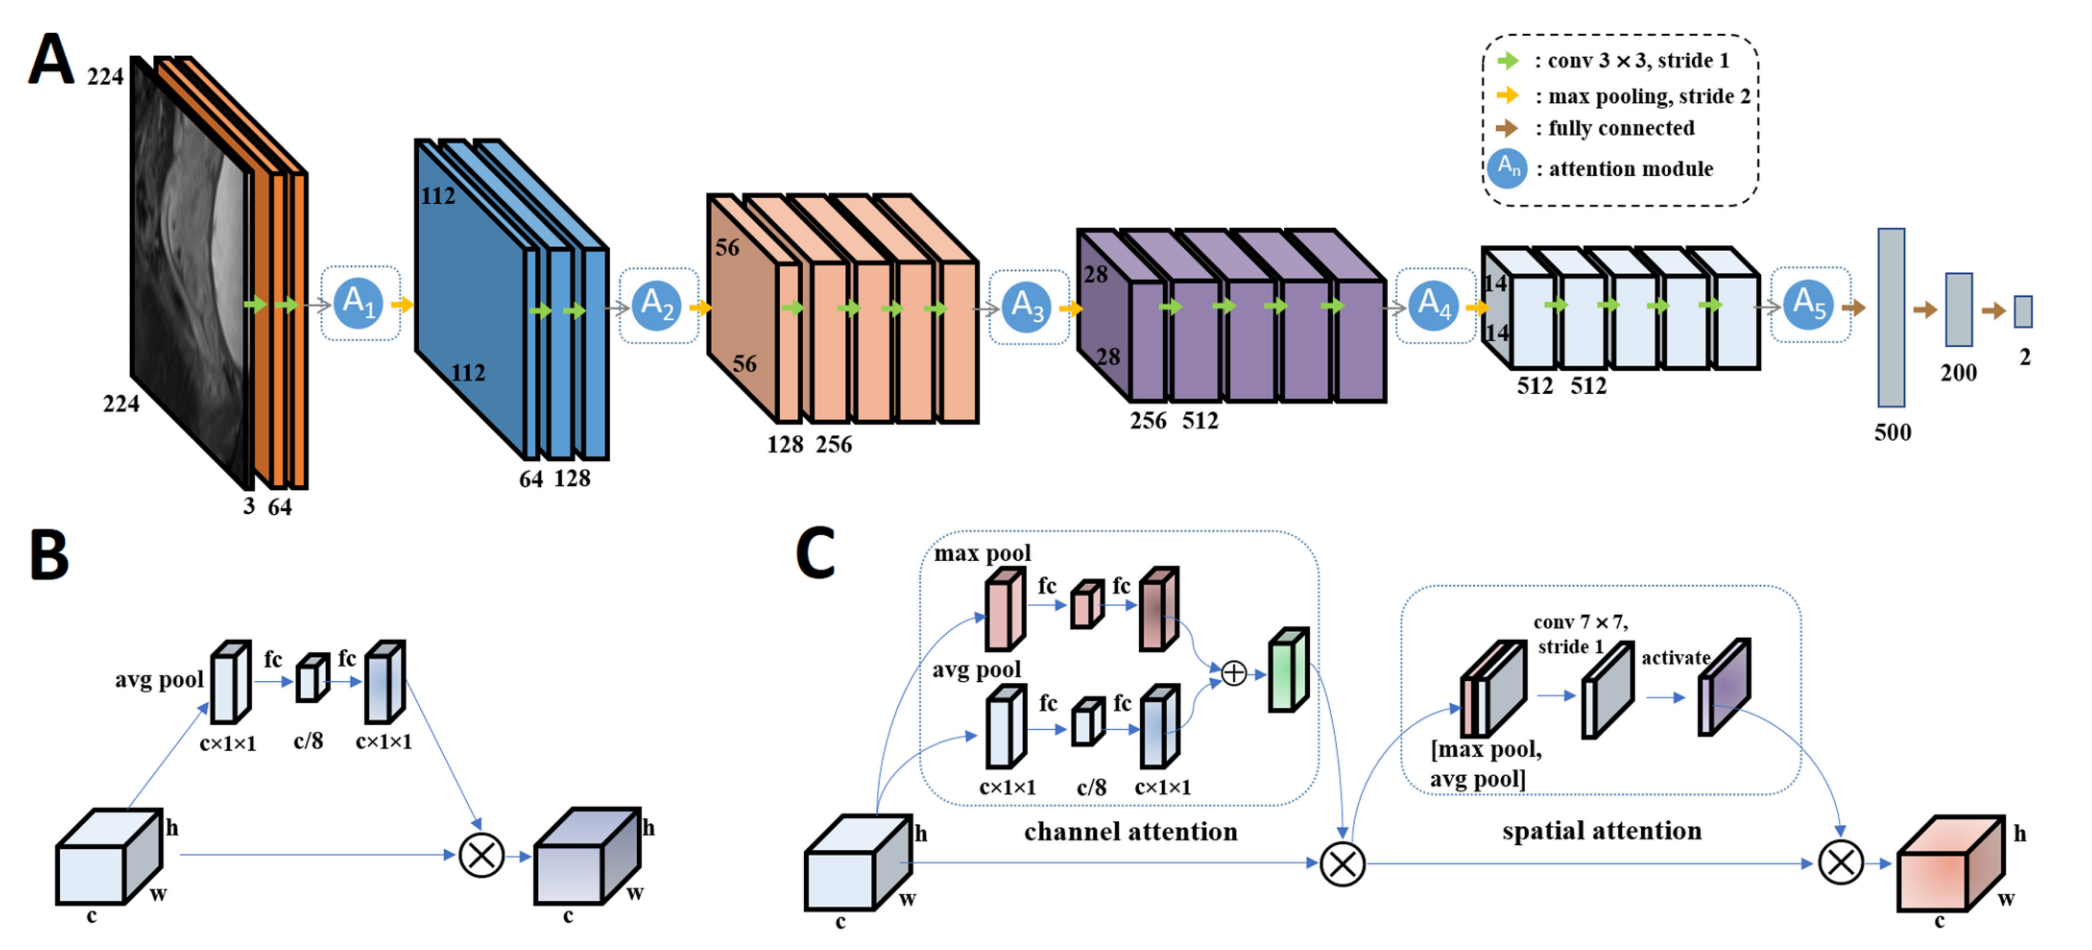
\includegraphics[width=0.8\textwidth]{figures/fig007.png}
    \caption*{Fonte: \cite{jiangMRIBasedRadiomics2021}}
    \label{fig:fig007}
\end{figure}

%---------------------------------------------------------
Em outro trabalho, \citeonline{renBiLSTMMultiheadAttentionbased2023}, desenvolveram um modelo avançado usando uma rede Bi-LSTM (memória de longo prazo bidirecional) combinada com um mecanismo de atenção de múltiplas cabeças, utilizando características radiômicas e imagens de \gls{TC} de lesões, para aprimorar a diferenciação dos principais subtipos de adenocarcinoma pulmonar, integrando assinaturas radiômicas com características radiológicas de tomografias computadorizadas. O estudo recrutou $421$ pacientes de três hospitais, confirmados com adenocarcinoma in situ, adenocarcinoma minimamente invasivo ou adenocarcinoma invasivo, com base na análise de $427$ lesões.

A metodologia empregada envolveu a extração de características radiômicas usando o software `\textit{PyRadiomics}' das regiões de lesões identificadas em cada imagem de \gls{TC}. As $100$ principais características foram então selecionadas através do método de classificação de características de máxima relevância e mínima redundância. Um modelo preditivo foi subsequentemente desenvolvido empregando essas características juntamente com as características radiológicas, usando a estrutura Bi-LSTM e atenção múltipla para classificar as lesões.

O desempenho diagnóstico do modelo foi quantitativamente impressionante, alcançando valores da área sob a curva (AUC) de $0,985$, $0,94$ e $0,981$ nos grupos de treinamento, teste e validação, respectivamente, com precisão correspondentes a $0,92$, $0,976$ e $0,91$. Além disso, comparações foram feitas com dois outros modelos — \gls{CNN} em conjunto com atenção múltipla, e LSTM em conjunto com atenção múltipla — demonstrando que o modelo Bi-LSTM e atenção múltipla superou essas alternativas em precisão e acurácia no conjunto de testes.

Esta pesquisa destaca a potente combinação de técnicas avançadas de aprendizado de máquina com análises radiômicas e radiológicas detalhadas para refinar o processo diagnóstico para subtipos de adenocarcinoma pulmonar, potencialmente orientando abordagens de tratamento mais personalizadas baseadas na caracterização do subtipo.

%---------------------------------------------------------
 \citeonline{aiSelfAttentionBasedFusion2023} conduziram um estudo inovador intitulado ``Um Modelo de Fusão Baseado em Autoatenção de Características Radiômicas e Profundas para Previsão de Recorrência Precoce em CPNP'', que aborda o significativo desafio de prever a recorrência precoce em câncer de pulmão de células não pequenas usando técnicas avançadas de aprendizado de máquina. Sua pesquisa aproveita o mecanismo de autoatenção para fundir características radiômicas manuais e características de aprendizado profundo extraídas de imagens de \gls{TC}, com o objetivo de aumentar a precisão preditiva e robustez para recorrência precoce em câncer de pulmão de células não pequenas.

O estudo começou empregando diversas técnicas de aprendizado de máquina para extrair uma variedade de características manuais de imagens de \gls{TC}, incluindo características de textura, forma e escala de cinza. Para capturar informações semânticas de alto nível e de representação, uma rede \textit{ResNet50} pré-treinada foi utilizada para a extração de características profundas. Essas características extraídas foram então fundidas com um vetor de características extraído de dados de texturas de imagens radiômicas e unificado usando um módulo de fusão de autoatenção inovador desenvolvido pelos pesquisadores. Este módulo otimiza e pondera o vetor de características fundidas, aproveitando plenamente o mecanismo de autoatenção para melhorar as capacidades de previsão do modelo e sua arquitetura pode ser conferida na Figura \ref{fig:fig008}.

Os resultados experimentais, avaliados no conjunto de dados público, \gls{TCIA}, demonstraram que o modelo proposto superou significativamente os métodos existentes na previsão de recorrência precoce. O modelo exibiu melhorias substanciais em precisão de classificação, sensibilidade, especificidade e \gls{AUC}, destacando seu potencial para guiar o tratamento em estágio inicial e melhorar as taxas de sobrevivência para pacientes com câncer de pulmão de células não pequenas.

Este estudo exemplifica a aplicação de técnicas avançadas de aprendizado de máquina em imagens médicas e oncologia, fornecendo um método robusto para a previsão de recorrência precoce que poderia impactar significativamente os resultados clínicos e as estratégias de tratamento em câncer de pulmão.

\begin{figure}[htbp]
    % \centering
    \caption{Arquitetura Proposta}
    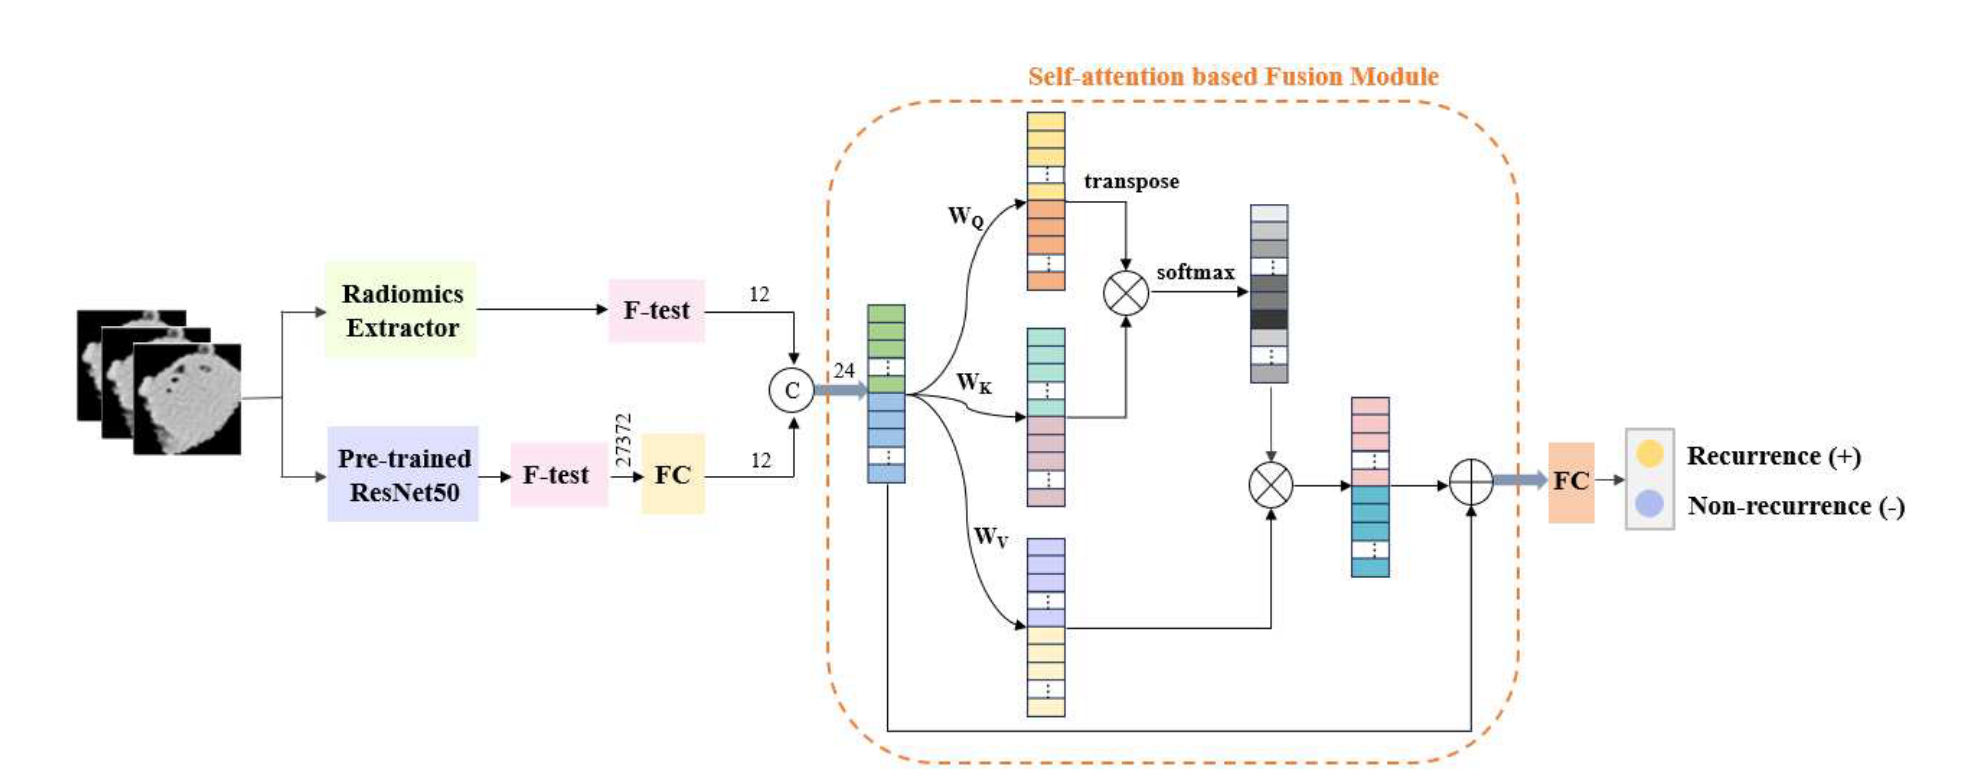
\includegraphics[scale=0.5]{figures/fig008.png}
    \caption*{Fonte: Adaptado de \citeonline{aiSelfAttentionBasedFusion2023}}
    \label{fig:fig008}
\end{figure}
%---------------------------------------------------------

\citeonline{iranmehrImprovedPredictionMGMT2022}
desenvolveram uma rede de aprendizado profundo inovadora que utiliza um mecanismo baseado em atenção para aprimorar a previsão do estado de metilação do gene MGMT em \gls{GBM}, o tipo mais agressivo de tumor cerebral. Pacientes com \gls{GBM} possuem uma expectativa muito baixa, entre 18 e 24 meses e requerem tratamentos agressivos, como por exemplo, quimioterapia. Sua pesquisa, apresentada em "\textit{Improved Prediction of MGMT Methylation Status in Glioblastoma using a Deep Attention Network}", destaca um avanço significativo nas capacidades diagnósticas não invasivas para \gls{GBM}, que tipicamente tem uma taxa de sobrevivência de apenas 18 meses.

O estudo foca no gene MGMT, cujo estado de metilação é crucial para determinar a eficácia da quimioterapia em pacientes com \gls{GBM}. As análises radiômicas tradicionais, embora úteis, muitas vezes não capturam os recursos intrincados necessários para uma previsão precisa da metilação. \citeonline{iranmehrImprovedPredictionMGMT2022} propõem um modelo que integra características radiômicas manuais com técnicas de \gls{AP}, melhorando a extração de características e a precisão da previsão de \gls{GBM}.

O modelo introduzido pela equipe utiliza uma combinação de mecanismos de atenção espremida e sequencial para priorizar fatias e regiões relevantes dentro das imagens de \gls{RMC}, respectivamente. Esse método não apenas melhora o foco em áreas significativas, mas também aprimora a interpretabilidade geral do modelo. O modelo proposto na Figura \ref{fig:fig009}, consiste de três etapas: 1) Um modelo base para extrair as características, 2) uma rede de atenção temporal e espacial e 3) uma rede de classificação para prever se o exame é metilado ou não metilado.
\newline

\begin{figure}[htbp]
    \centering
    \caption{Método proposto. \textit{DenseNet} é o modelo base, a saída da rede densa é alimentada pela rede de atenção que prioriza as fatias e regiões e gera a classificação binária do status de metilação do MGMT.
    }
    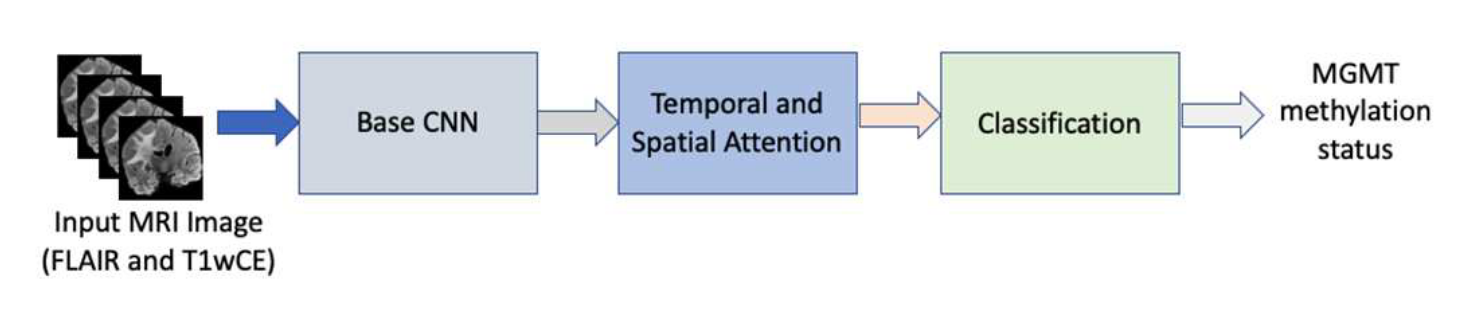
\includegraphics[width=1\textwidth]{figures/fig009.png}
    \caption*{Fonte: Adaptado de \cite{iranmehrImprovedPredictionMGMT2022}}
    \label{fig:fig009}
\end{figure}

O modelo base consiste em uma \textit{DenseNet} e segundo o autor, ela pode suportar milhares de camadas e ser resistente ao \textit{overfitting}. A saída da rede densa é fornecida para a rede espremida e autoatenção conforme mostrado na Figura \ref{fig:fig010}. Cada exame consiste em várias fatias e a atenção espremida priorizará fatias, usando o \textit{average pooling} global seguido por duas camadas densas separadas e depois o produto escalar com a entrada inicial. A saída da atenção espremida é fornecida à rede de autoatenção. Após a aplicação da autoatenção, o mapa de atenção contém \textit{pixels} com uma seção de maior importância em cada fatia. Com a rede de autoatenção, é possível enfatizar \textit{pixels} e regiões diferentes independente da distância em que estes \textit{pixels} se localizam na imagem. Múltiplas regiões com diferentes tamanhos, geradas a partir de regiões integrais, são então fornecidas à atenção sequencial. A rede de atenção sequencial adapta uma rede \gls{LSTM}, que é capaz de aprender dependências de longo prazo. A saída passa por uma camada densa e uma função sigmoide para fins de classificação.

Avaliado em várias métricas de classificação binária, o modelo alcançou a melhor \gls{AUC} de 70,59, demonstrando sua superioridade em relação aos métodos existentes. Este trabalho fornece uma abordagem robusta e automática para capturar características críticas de imagens de ressonância magnética, avançando significativamente na previsão do estado de metilação em \gls{GBM} em comparação com métodos anteriores. As implicações de tais avanços são profundas, potencialmente melhorando o planejamento de tratamentos personalizados e, em última análise, os resultados para os pacientes com glioblastoma.

\begin{figure}[htbp]
    \centering
    \caption{Arquitetura Proposta}
    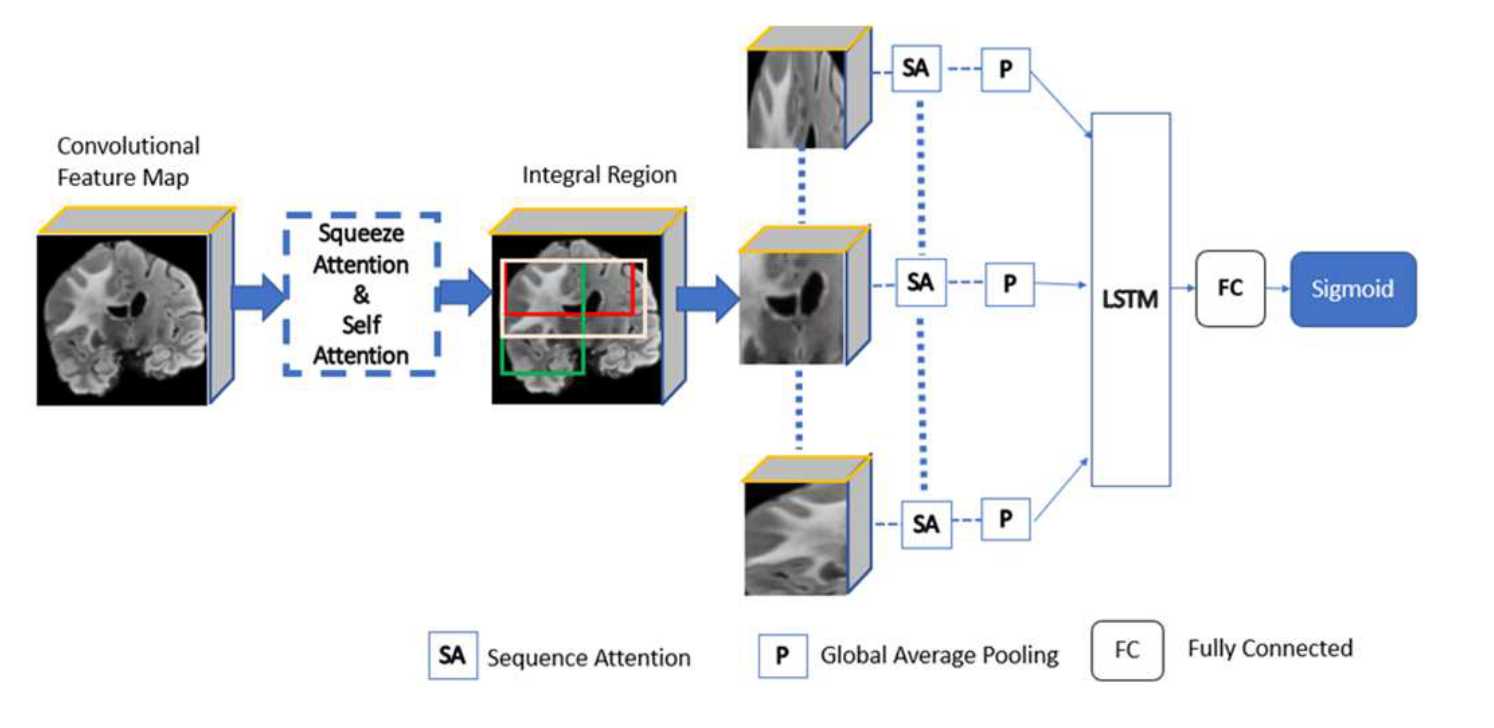
\includegraphics[width=1\textwidth]{figures/fig010.png}
    \caption*{Fonte: Adaptado de \cite{iranmehrImprovedPredictionMGMT2022}}
    \label{fig:fig010}
\end{figure}

\noindent \textcolor{red}{
< < --- ADC. TRAB. QUE DEMONSTRA VÁRIOS MECANISMOS DE ATENÇÃO ----
}

Por fim, \citeonline{yangNeuralNetworkDesign2024a} demonstra como o mecanismo de atenção auxilia as redes neurais a se concentrar em informações pertinentes nos dados, e sua integração com redes neurais convolucionais aprimora as capacidades de extração de características do modelo como um todo. O trabalho destaca que o mecanismo de atenção pode ser ser categorizado em: mecanismo de atenção seletiva e mecanismo de autoatenção.

O mecanismo de atenção seletiva gera um conjunto de pesos de atenção ao prever diretamente a importância de cada parte dos dados em relação ao objetivo da tarefa, adicionando os pesos ponderadamente aos dados de entrada para realçar as informações importantes e suprimir as informações irrelevantes nos dados. A \gls{SE}Net é um trabalho representativo nos mecanismos de atenção seletiva. A \gls{SE}Net propõe um mecanismo de atenção no domínio dos canais que aprende o valor dos pesos para cada canal no mapa de características, a fim de realçar ou suprimir cada característica do canal. O mecanismo de atenção seletiva é orientado para os objetivos da tarefa e otimiza diretamente as características, mas carece da capacidade de extrair informações globais. O mecanismo de autoatenção consegue capturar informações globais, mas sofre com alta complexidade e dificuldades de otimização. 

\citeonline{yangNeuralNetworkDesign2024a} propuseram um algoritmo com módulo de busca de atenção diferenciável, assim a rede pode extrair as informações cognitivas e semântica das características da imagem. Em seguida, um espaço de busca multi-atenção é estabelecido englobando seis operações de atenção consolidadas em um único módulo de busca. Por fim, para aprimorar a eficiência, o espaço de busca, antes discreto, é convertido para contínuo, empregando um algoritmo de busca diferencial para identificar a rede de atenção ótima. Para validar os resultados, foi aplicada a classificação em imagens  muito detalhadas. A Figura \ref{fig:fig022} e \ref{fig:fig023} demonstram respectivamente a arquitetura proposta no trabalho e o módulo de busca multi-atenção.
\newline

\textcolor{red}{
-------------------------------------------------------------------------------------------- > >
}

\begin{figure}[htbp]
    \centering
    \caption{Arquitetura Multi-Atenção Proposta}
    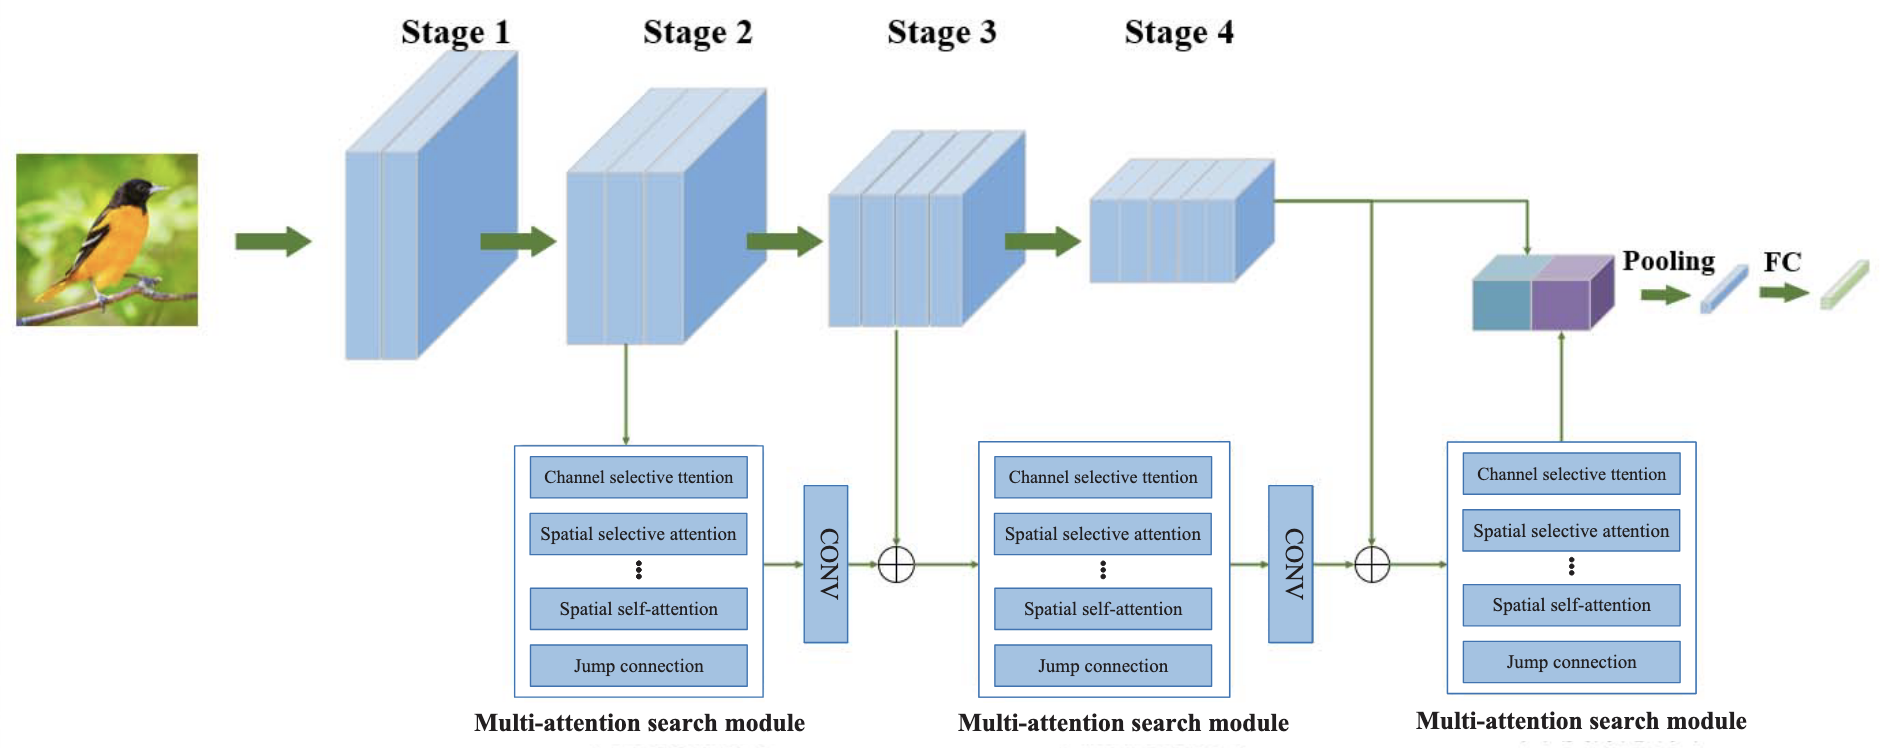
\includegraphics[width=1\textwidth]{figures/fig022.png}
    \caption*{Fonte: \cite{yangNeuralNetworkDesign2024a}}
    \label{fig:fig022}
\end{figure}

\begin{figure}[htbp]
    \centering
    \caption{Módulo Multi-Atenção}
    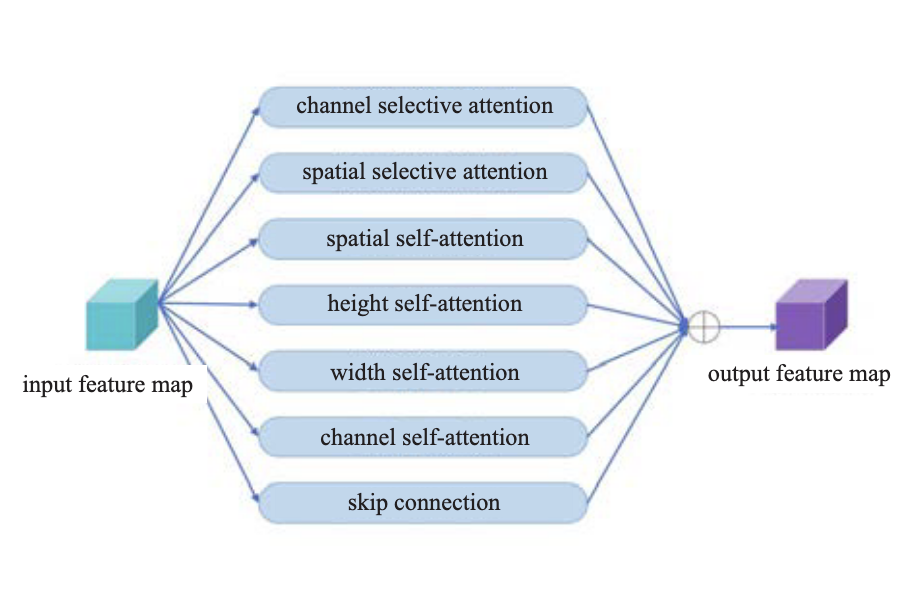
\includegraphics[width=1\textwidth]{figures/fig023.png}
    \caption*{Adaptado de \cite{yangNeuralNetworkDesign2024a}}
    \label{fig:fig023}
\end{figure}
%---------------------------------------------------------
% \section{Considerações Finais do Capítulo}
% \label{sec:rcond_cap_3}
% \lipsum[2-4]